% Created 2022-04-15 Fri 02:45
% Intended LaTeX compiler: pdflatex
\documentclass[12pt]{extarticle}
\usepackage[utf8]{inputenc}
\usepackage[T1]{fontenc}
\usepackage{graphicx}
\usepackage{longtable}
\usepackage{wrapfig}
\usepackage{rotating}
\usepackage[normalem]{ulem}
\usepackage{amsmath}
\usepackage{amssymb}
\usepackage{capt-of}
\usepackage{hyperref}
\usepackage{minted}
\usepackage[french]{babel}
\usepackage{tree-dvips}
\usepackage{titlesec}
\usepackage{fontspec}
\usepackage[top=2.54cm, bottom=2.54cm, left=1.91cm, right=1.91cm]{geometry}
\usepackage{graphicx}
\usepackage{setspace}
\usepackage{tikz}
\usepackage{hyperref}
\usepackage{xcolor}
\usepackage{float}
\usepackage{listings}
\usepackage{minted}
\usepackage[font=bf, skip=2pt]{caption}
\usepackage[most,listings]{tcolorbox}
\usepackage[style=apa] {biblatex}
\usepackage{xurl}
\usepackage{subfig}

\defaultfontfeatures{Mapping=tex-text,Scale=MatchLowercase}
\setmainfont{Open Sans}
\setmonofont{Consolas}
\floatstyle{plaintop}
\restylefloat{table}
% \titleformat{\paragraph}
% {\normalfont\normalsize\bfseries}{\theparagraph}{1em}{}
% \titlespacing*{\paragraph} {0pt}{3.25ex plus 1ex minus .2ex}{1.5ex
%   plus .2ex}

% \titlespacing{\section}{0pt}{\parskip}{-\parskip}

\graphicspath{{./img/}}

% \tcbset{colframe=white}

\hypersetup{
  colorlinks,
  linkcolor={red!50!black},
  citecolor={blue!50!black},
  urlcolor={blue!80!black}
}

\lstset{
  basicstyle=\ttfamily,
  backgroundcolor=\color{gray},
  showstringspaces=false,
  commentstyle=\color{red},
  keywordstyle=\color{blue}
}

\definecolor{monokaibg}{HTML}{272822}
\definecolor{borlandbg}{HTML}{eeeeee}
\definecolor{sectionbg}{HTML}{56b0c9}
\definecolor{titlepagebg}{HTML}{44899d}
% \definecolor{Text}{HTML}{FFFFFF}
% \AtBeginEnvironment{minted}{\color{Text}}

\newcommand{\csection}[1]{
  \begin{tcolorbox}[colback=sectionbg]
    \section{#1}
  \end{tcolorbox}
  \noindent
}


\newcommand{\titre}[1]{
\vfill
\begin{spacing}{1.2}
\huge\textsc{#1}
\end{spacing}
\vfill
}
\newcommand{\cours}[1]{{\Large\textsc{#1}}}
\newcommand{\groupe}[1]{{\Large #1}}

\newenvironment{ctitlepage}
{\cleardoublepage\begin{titlepage}\thispagestyle{empty}\begin{center}
      
\includegraphics[scale=1]{polylogo.png}
      \vfill}
    {\end{center}\end{titlepage}}

\onehalfspacing
\addbibresource{template.bib}
\let\cite\parencite
\nocite{*}
\date{}
\title{Template}
\begin{document}

\begin{ctitlepage}

\cours{INF8215}

\groupe{Groupe 01}

\titre{\textbf{TP3} \\
Classifications multiclasses:\\
légumes secs}

\vspace{.1in}

\textbf{Par} \\
Brando, Tovar \textbf{1932052} \\
Vega, Estefan \textbf{1934346} \\
Équipe: \textbf{BrandiniStifini} \\

\vspace{.5in}

Le \today

\end{ctitlepage}

\newpage
\tableofcontents
\newpage


\section{Contexte}
\label{sec:orgfbb2c37}
Dans ce travail pratique, il nous était demander de classifier des légumes secs dans leur catégorie respectives. Il y en avait 7 en tout; Sira, Horoz, Dermason, Barbunya, Cali, Bombay, Seker et nous devions déterminer la catégorie à l'aide de 16 \emph{features}. Nous avions donc à résoudre un problème de classification multiclasses. Nous avons décider d'utiliser la librairie \emph{scikit-learn} et le modèle que nous avons utilisé se base sur les machines à vecteurs de support (\emph{SVC OneVsOneClassifier}). Nous avons aussi exploré d'autres modèle telles que celui basée sur la descente de gradient stochastique (\emph{SGDClassifier}) et celle basée sur les forêts aléatoires (\emph{RandomForestClassifier})

\section{Prétraitement}
\label{sec:org254594a}
Avant de commencé à résoudre le problème, il est utile de se familiariser avec les données. Nos données étaient constitué de 16 \emph{features}. Il y avait 6000 données de test. Nous avons commencé par voir s'il manquait des valeurs dans certaines de no données test ce qui n'était pas le cas. Nous avons ensuite regardé si nos donées étaient balancées.
\vspace{5mm}

\begin{minipage}{.45\textwidth}
\captionof{figure}{Diagramme à bandes des catégories}
\vspace*{-5mm}
\begin{center}
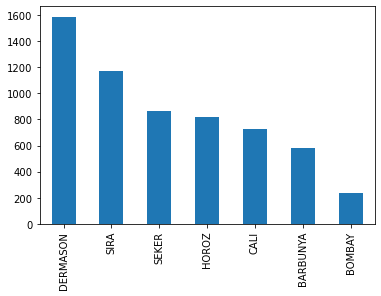
\includegraphics[width=\linewidth]{./.ob-jupyter/0e36c24725fa023c6e39f07bc9df640645c86811.png}
\end{center}
\label{fig:barchart}
\end{minipage}
\begin{minipage}{.55\textwidth}
\captionof{figure}{Matrice de corrélation}
\vspace*{-5mm}
\begin{center}
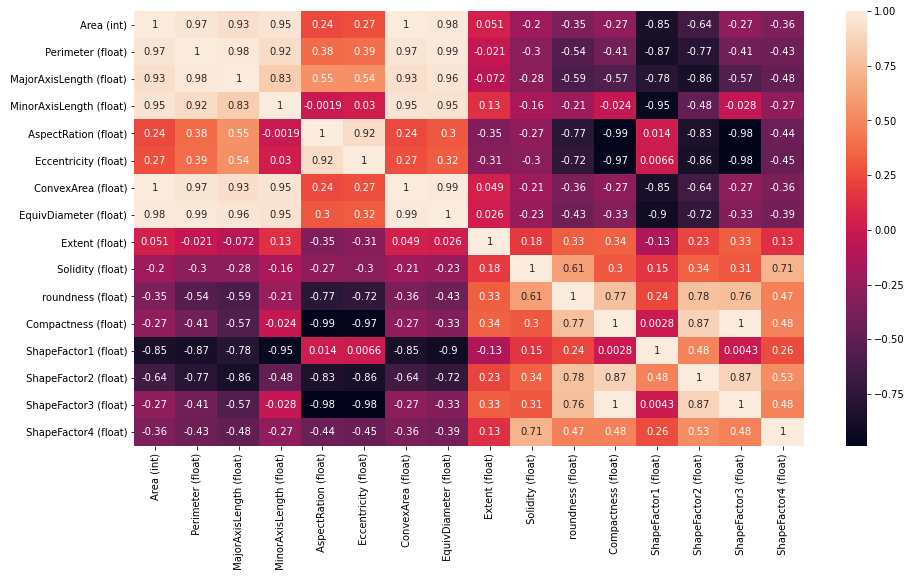
\includegraphics[width=\linewidth]{./.ob-jupyter/da88383af5d1618a3cb0bf8008eb6ce0c4c86bce.png}
\end{center}
\label{fig:heatmap}
\end{minipage}

\vspace{5mm}

Il a été intéressant de voir qu'il y a présence de débalancement (\hyperref[fig:barchart]{figure 1}) et que certains attributs étaient très corrélés entre eux soit > 0.9 ou < -0.9 (\hyperref[fig:heatmap]{figure 2}). Nous avons essayer de retirer les attributs corrélées, mais il n'y a pas vraiment eu de gain et nous avons donc décider de garder tous les attributs.

Une fois les analyse de données terminées, nous avons dû faire quelques changement dans les données afin de pouvoir utiliser notre modèle. Nous avons en premier lieu, dû transformer les valeurs de X\_train (attributs) en float. Nous avons ensuite retirer les valeurs de \emph{ID} dans X\_train et y\_train. Nous pouvions ainsi entrainer notre modèle. Étant données les mauvais résultats initiaux, nous avons dû faire appel à la normalisation. Nous sommes donc passées d'une précision de 0.268 à une de 0.933 sur le classificateur SVM. Le \emph{scaler} qui a donné les meilleurs résultats est le \emph{StandardScaler} de \emph{scikit-learn}.

\section{Méthodologie}
\label{sec:org843d733}
Le classificateur que nous avons choisis (\emph{SVC}) est un classificateur binaire. Il était donc nécessaire de combiner ce classificateur avec une autre méthode. Nous avons donc choisi la méthode OneVsOne (/OneVsOneClassifier). En combinant ces deux algorithmes, nous obtenons un classificateur multiclasses qui est en fait composées de plusieurs classificateurs binaire. Dans notre cas nous avons 7 * 6 / 2 = 21 classificateurs binaires aux total.

En ce qui concerne la répartition des données, nous avons utilisé l'intégralité des données pour tester notre modèle. Nous avons pris cette décision, car nous avons utilisé en parallèle la méthode de vérification \emph{k-fold cross-validation} avec k = 10. Ainsi, les données sont diviser en 10 parties dont 9 sont utilisées pour l'entraînement et la dernière comme partie de validation.

Comme nous pouvons le voir à la figure \hyperref[fig:barchart]{figure 1}, nos données étaient assez débalancées. Nous avons fait des recherches à ce sujet et il y avait plusieurs solutions possibles. Il y avait la possibilité de faire du \emph{oversampling} et du \emph{undersampling}. Nous n'avons malheureusement pas eu de succès avec ces deux méthodes. Étant donnée que nous avons utilisés le modèle \emph{SVC} de scikit-learn, nous avions accès a l'hyperparamètre \emph{class\textsubscript{weight}} avec comme valeur \emph{balanced} qui associe un poids à chaque classe selon sa fréquence dans les données pour gérer les débalancements. Malheureusement cet hyperparamètre n'a pas impacté positivement nos résultats.

Le modèle que nous avons utilisé est basé sur les machines à vecteurs de support et il y a deux paramètres principaux à tenir en compte, \emph{C} et \emph{gamma}. D'abord il est utile de comprendre que ce modèle classifie les données de façon linéaire et que pour classifier des données de non linéaires, la méthode utilise une fonction applé noyau (\emph{kernel}). La valeur du gamma détermine à quel point les points proche et loin de la délimitation ont de l'importance. En d'autre mots, des valeurs élevé de gamma auront une meilleur délimitation, avec plus de curvatures, entre les données et donc le modèle aura plus tendance à souffrir de sur-apprentissage. À l'inverse, des
\begin{minipage}{.45\textwidth}
\vspace*{2.5mm}
valeurs faibles de gamma nous mèneront plus vers un problème de sous-apprentissage. La valeur de C nous indique plutôt notre niveau de tolérance aux erreurs et sa valeur impactera sur la généralisation de notre modèle. Une grande valeur de C augmente la precision et reduit les erreurs. Il fallait donc trouver un équilibre entre la précision de notre de modèle sur le données d'entrainement et sa capacité a généraliser. Nous avons trouver un équilibre optimale avec le valeur \emph{gamma} = 0.19 et \emph{C} = 2.8. Les impacts de ses paramètres peuvent être observés sur la \hyperref[fig:svm_c_gamma]{figure 3} \cite{support_vector_machines}.
\end{minipage}
\begin{minipage}{.55\textwidth}
\vspace*{1mm}
\captionof{figure}{SVM paramètres C et gamma}
\vspace*{-5mm}
\begin{center}
\includegraphics[width=\linewidth]{./img/svm_c_gamma.png}
\end{center}
\label{fig:svm_c_gamma}
\end{minipage}


\section{Résultats}
\label{sec:org6f48b26}
Nous avons pris notre décision sur le classificateur avant tout selon la précision avec les hyperparamètres par défauts. Le \hyperref[classificators]{tableau 1} montre les résultats des 3 classificateurs testés avec leurs hyperparamètres par défaut.
\vspace{2mm}
\captionof{table}{Comparaison des classificateurs testés avec k-fold cross-validation k=10}
\vspace*{-5mm}
\label{classificators}
{\scriptsize
\begin{center}
\begin{tabular}{|l|r|r|r|r|r|r|r|r|r|r|r|r|}
\hline
Classificateur & 1 & 2 & 3 & 4 & 5 & 6 & 7 & 8 & 9 & 10 & \textbf{Moyenne} & \textbf{Training set accuracy}\\
\hline
SVC OneVsOneClassifier & 0.935 & 0.938 & 0.913 & 0.937 & 0.928 & 0.923 & 0.925 & 0.947 & 0.93 & 0.923 & 0.93 & 0.935\\
\hline
RandomForestClassifier & 0.923 & 0.923 & 0.898 & 0.933 & 0.925 & 0.898 & 0.908 & 0.933 & 0.918 & 0.912 & 0.917 & 1.0\\
\hline
SGDClassifier & 0.915 & 0.92 & 0.902 & 0.94 & 0.91 & 0.885 & 0.922 & 0.932 & 0.922 & 0.903 & 0.915 & 0.92\\
\hline
\end{tabular}
\end{center}
}
\setlength\parindent{20pt}Nous voyons qu'avec les hyperparamètres par défauts c'est bien le classificateur SVC qui donne les meilleurs résultats.

Finalement, nous avons optimisé notre classificateur avec \emph{gamma} = 0.19 et \emph{C} = 2.8 et avons comparé les différents \emph{scalers}. Le \hyperref[scalers]{Tableau 2} montre les résultats sur les différents scalers testés.
\vspace{2mm}
\captionof{table}{Comparaison des scalers testés avec k-fold cross-validation k=10}
\vspace*{-5mm}
\label{scalers}
{\scriptsize
\begin{center}
\begin{tabular}{|l|r|r|r|r|r|r|r|r|r|r|r|r|}
\hline
Classificateur & 1 & 2 & 3 & 4 & 5 & 6 & 7 & 8 & 9 & 10 & \textbf{Moyenne} & \textbf{Training set accuracy}\\
\hline
StandardScaler & 0.938 & 0.947 & 0.92 & 0.94 & 0.927 & 0.932 & 0.92 & 0.952 & 0.93 & 0.925 & 0.933 & 0.944\\
\hline
MinMaxScaler & 0.927 & 0.928 & 0.89 & 0.933 & 0.925 & 0.915 & 0.918 & 0.935 & 0.927 & 0.918 & 0.922 & 0.924\\
\hline
MaxAbsScaler & 0.907 & 0.922 & 0.872 & 0.913 & 0.917 & 0.903 & 0.905 & 0.927 & 0.913 & 0.902 & 0.908 & 0.91\\
\hline
Sans normalisation & 0.27 & 0.268 & 0.268 & 0.265 & 0.268 & 0.265 & 0.27 & 0.272 & 0.267 & 0.27 & 0.268 & 1.0\\
\hline
Normalizer & 0.263 & 0.263 & 0.263 & 0.265 & 0.265 & 0.265 & 0.265 & 0.265 & 0.265 & 0.263 & 0.264 & 0.264\\
\hline
\end{tabular}
\end{center}
}

\section{Discussion}
\label{sec:orgc543904}
\setlength\parindent{20pt}Les modèle que nous avons testés étaient tous simple d'implémentation avec \emph{scikit-learn}. Ce qui était un peu plus difficil était d'ajuster les différents paramètres et de normaliser correctement les données, afin d'avoir un résultat optimal. Nous sommes assez satisfaits des résultats de notre modèle qui, sur kaggle donne une précision de \textbf{0.932}. En théorie, le modèle SVM est susceptible aux grands débalancements des données. Malgré cela, ne pas en tenir compte s'est avéré être le plus bénéfique pour nous. Le modèle SVM n'est aussi pas optimales pour gérer une grande quantité de données tests. En effet, SVM utilise une matrice noyau dont la taille est proportionnelle à la quantité de données test ce qui affecte les performances.

Il y a tout de même plusieurs avantages à utiliser le modèle SVM, notamment, l'utilisateur a beaucoup de contrôle sur celui-ci. Il y a d'abord les paramètres \emph{gamma} et \emph{C} qui permet a l'utilisateur de gérer le sur et sous-apprentissage. Mais il y a surtout le paramètre \emph{kernel} qui permet à l'utilisateur d'utiliser sa propre matrice pour un utilisateur qui aurait des connaissances expertes sur ses données \cite{sklearn}.

En ce qui concerne notre travail, il nous a pas été trop difficile de trouver des paramètres adequa afin de gérer le sur-apprentissage. Même avec les paramètres par défaut nous avions un très bon modèle qui n'avait pas beaucoup de sur-apprentissage. Par contre, il est intéressant de voir que le classificateur \emph{RandomForestClassifier} avait un \emph{training accuracy} de 1.0 alors qu'avec la \emph{cross-validation} il n'obtenais que 0.917 de précision.

\newpage
\phantomsection
\addcontentsline{toc}{section}{Références}
\printbibliography
\end{document}
